\section{The \textsc{G-Eagle} Simulations}

We will now detail our simulations, including the selection of the regions and the zoom resimulation technique.
Details of the \textsc{Eagle} physics model are provided in \cite{schaye_eagle_2014,crain_eagle_2015}.

\subsection{Region Selection}

\begin{figure}
	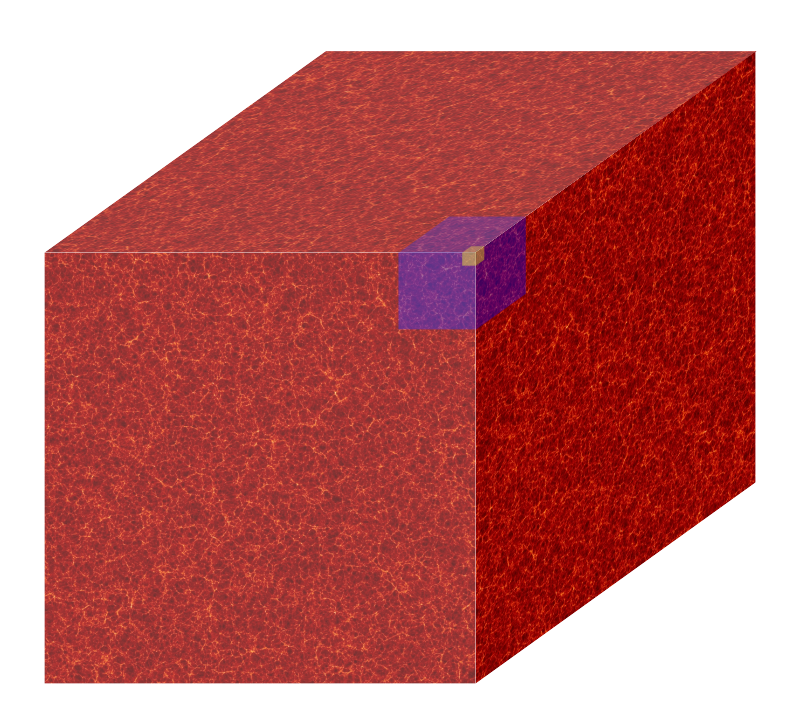
\includegraphics[width=\columnwidth]{images/3D_L3200.png}
    \caption{Diagram of the $3.2 \; \mathrm{Gpc}$ box from which we select our regions. To demonstrate the increase in volume, we show the Bluetides simulation \protect\citep[$L = 500 \;\mathrm{cMpc}$;][]{feng_bluetides_2015} inset in blue, and the fiducial EAGLE simulation \protect\citep[$L = 100 \; \mathrm{cMpc}$;][]{schaye_eagle_2014} inset in yellow.}
    \label{fig:L3200}
\end{figure}

We use the same parent simulation as that used in the \textsc{C-Eagle} simulations \citep{barnes_redshift_2017}, a $(3.2 \; \mathrm{Gpc})^3$ dark matter-only simulation with a particle mass of $8.01 \,\times\, 10^{10} \; M_{\odot}$.
\fig{L3200} shows a diagram of the box compared to the fiducial \textsc{Eagle} reference volume, as well as the \textsc{Bluetides} simulation \citep{feng_bluetides_2015}.
The highest redshift snapshot available for this simulation is at $z = 4.67$, which we use for our selection.
Regions will not necessarily remain in rank ordering in overdensity space when extending to higher redshifts; we discuss this in greater detail in Section \todo{????}.

In order to reduce the surface area exposed to the low resolution dark matter only region we choose a spherical high resolution region.
Given a chosen radius for the sphere, it is then necessary to calculate the density within spheres throughout the parent volume in order to select regions with the desired overdensity.
We approximate the density by first finding the mass on a high resolution grid through a nearest grid point assignment  scheme, then find the density on arbitrary scales by convolving the grid with a top-hat spherical filter.
We choose a grid with spacing of 2.6 Mpc, and a sphere with radius 14 Mpc.\footnote{code provided at \\\href{https://github.com/christopherlovell/DensityGridder}{https://github.com/christopherlovell/DensityGridder}}
We found that this gives a density very close to the `truth' calculated from the raw particle data.

\begin{figure}
	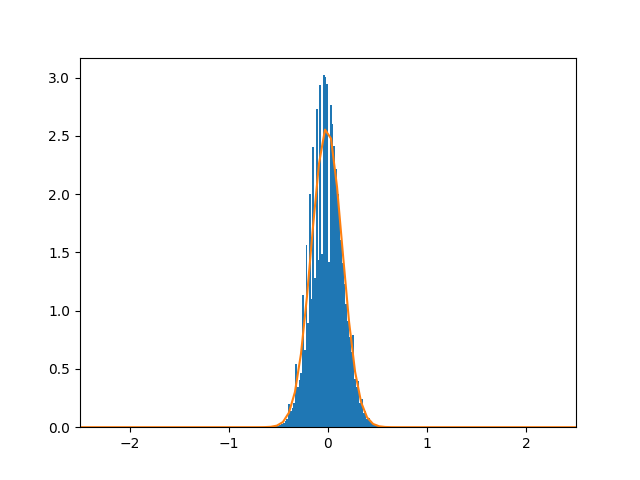
\includegraphics[width=\columnwidth]{images/log_fit.png}
    \caption{Log-normal distribution of overdensities}
    \label{fig:log_fit}
\end{figure}

The overdensity is then defined as
\begin{equation}
	\delta(\textbf{x}) = \frac{\rho(\textbf{x})}{\langle \, \rho(\textbf{x}) \, \rangle} - 1 \;\;,
\end{equation}
where $\rho$ is the density at grid coordinates $\textbf{x}$.
\fig{log_fit} shows the distribution of overdensity in log-space, alongside a fitted log-normal distribution.
We select regions of a given overdensity by selecting a narrow range of overdensity around the desired value, then randomly select a region of this overdensity.
We test to ensure the selected region does not overlap with any previously selected region.
The selected regions are listed in \app{regions}.


\begin{figure}
	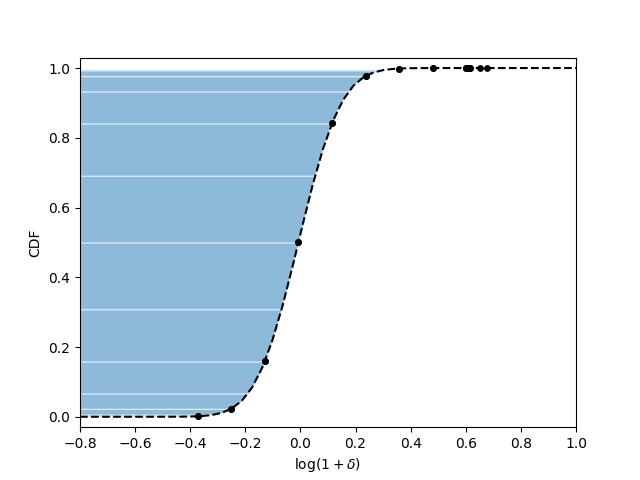
\includegraphics[width=\columnwidth]{images/CDF.png}
    \caption{Cumulative distribution function of overdensities in the parent volume.}
    \label{fig:CDF}
\end{figure}

\subsection{Resimulation}


\begin{table}
	\centering
	\caption{Variation of subgrid parameters between models. }
	\label{tab:example_table}
	\begin{tabular}{lcccc}
		\hline
		\textbf{Simulation Prefix} & $n_{H,0}$ & $n_{n}$ & $C_{\mathrm{visc}}$ & $\Delta T_{\mathrm{AGN}}$\\
		\hline
     & $\mathrm{[cm^{-3}]}$ & & & $\mathrm{[K]}$ \\
		\hline
		Ref & 0.67 & $2/ln(10)$ & $2 \pi$ & $10^{8.5}$ \\
		AGNdT9 & 0.67 & $2/ln(10)$ & $2 \pi \times 10^{2}$ & $10^{9}$ \\
		\hline
	\end{tabular}
\end{table}


\todo{update so not identical to c-eagle paper}
We use the AGNdT9 configuration of the \textsc{Eagle} parameters.
This is identical to that used in the \textsc{C-Eagle} simulations, but differs from the fiducial Reference simulation (see \tab{example_table}); it uses a higher value for $C_{\mathrm{visc}}$, which controls the sensitivity of the BH accretion rate to the angular momentum of the gas, and a higher gas temperature increase from AGN feedback, $\Delta T$.
A larger $\Delta T$ leads to fewer, more energetic feedback events, whereas a lower $\Delta T$ leads to more continual heating.
We use an identical resolution to the fiducial \textsc{Eagle} simulation, with gas particle mass $m_{g} = 1.8 \times 10^6 \; \mathrm{M_{\odot}}$, and a physical softening length of $0.7 \; \mathrm{kpc}$.


Galaxies on the edge of the high resolution region will not be modelled correctly due to the presence of a pressureless boundary.
To avoid this we resimulate a region 15 Mpc in radius, and ignore all galaxies within 1 Mpc of the edge of the sphere in post-processing.
Excluding galaxies on the boundary at higher redshifts, where the region becomes aspherical, is described in \sec{post_proc}.

\subsection{Post-processing}
\label{sec:post_proc}



We therefore use a sphere as our simulation volume, as this has the largest ratio of volume to surface area, reducing the volume of our simulation we eventually discard.
At higher redshift the high resolution region deforms, which makes the spherical symmetry assumption invalid.
In this case we find the radius to the most distant particle from the box centre.


We limit our analysis to galaxies sampled by at least 100 star particles, \textit{e.g.} $\mathrm{log_{10}(M_{*}\,/\,M_{\odot})} \geqslant 8.25$.

\todo{state number of galaxies, compare to periodic volumes}

\subsection{Distribution Function Weighting}

\fig{CDF} shows the cumulative distribution function of log overdensity, $\mathrm{log}(1 \,+\, \delta)$.
Each point on the CDF curve shows a selected region.
We make the following assumption: that regions of a given overdensity $\delta_{A}$ will be similar to nearby overdensities ($\delta_{A}\,-\, \Delta_{1}$, $\delta_{A}\,+\, \Delta_{2}$).
We can therefore assume that all other regions with overdensity in this range can be represented by the given resimulated region.
We choose $\Delta_{1}$ and $\Delta_{2}$ to bisect the distance in overdensity space between the given region and the nearest neighbouring region ($\delta_{B} \,<\, \delta_{A}$) in overdensity space,
\begin{equation}
	\Delta_{1} = \frac{\delta_{A} + \delta_{B}}{2}
\end{equation}


Where there are multiple regions of a similar overdensity, \textit{e.g.} at the high overdensity end, we group regions together to represent an extended range of overdensity space. This ensures that given regions are not unfairly weighted low by virtue of having nearbgy regions in overdensity space.
The weights for each region are quoted in \app{regions}.
